\chapter{Event Reconstruction}\label{chapt:event_selection}

Any physics analysis operates particles and their features. Thus one of the essential tasks on the way to a physical
result is to interpret outcoming detector data as a set of physical objects making use of the hits
in the tracker, energy deposits in the calorimeter and signals from the muon system. Assigning this information to some concrete particle 
or object is a reconstruction procedure.

Different algorithms and methods are used to reconstruct different objects and some of them (relevant for this analysis -- leptons, jets and missing transverse
energy, responsible for neutrinos) are discussed in this
chapter. In general, for this analysis each object of the $t\bar{t}$ dileptonic final state was reconstructed using the information from many
CMS sub-detectors.

%%%%%%%%%%%%%%%%%%%%%%%%%%%%%%%%%%%%%%%%%%%%%%%
\section{Track and Vertex Reconstruction}
 
Tracks \footnote{A \textit{track} is a set of information about the charged particles trajectory curve and momentum.} and vertecies 
\footnote{A \textit{vertex} is an estimate of a point in space where the particles arise from. It can be either related to the 
collision point or to the place  where some secondary interaction happened.} are the essential objects used for all the particles reconstruction. 
But they are also not the primer detector output and they have to be reconstructed.

\subsection{Track Reconstruction}

First, the track reconstruction has to take place, using the information from the inner tracking detectors. The pixel and strip detectors 
produce signals, which are grouped to clusters. A position of a cluster, or a hit, is an estimate of the point where a particle crossed the
detector material. In simple words a particle trajectory can be tracked if fitting the corresponding consequence of hits. A curvature 
of the trajectory with the known magnetic field gives a momentum estimate of a particle.

A track reconstruction is an iterative process in which first the "easiest" trajectories are reconstructed (e.g. the ones with the highest
transverse momentum or those, which are produced in the primary interaction region). The hits used for a particular track reconstruction 
are not used for any other track definition. After the number of hits is reduced in the first iterations, it is easier to reconstruct the
tracks from the other more problematic particles (e.g. low-momentum or very displaced from the primary interaction region). Each track is reconstructed
following the sequential steps \cite{Chatrchyan:2014fea}:

\begin{itemize}
 \item \textbf{Seed generation}: provides initial, hypotetical, track candidates. Assuming helical path of the particles in the
 quasi-uniform magnetic field, a set of parameters for the trajectory is defined either using 3 hits or 2 hits and the assumption
 of the track origin (close to the primary interaction region\footnote{A primary interaction region or a \textit{beam spot} is defined 
 as an a}).
\end{itemize}


% 
% %%%%%%%%%%%%%%%%%%%%%%%%%%%%%%%%%%%%%%%%%%%%%%%
% \section{Particle Flow Concept}\label{sec:PF}
% 
% All the objects in $t\bar{t}$ dileptonic final state were reconstructed making use of \textit{Particle Flow} (PF)
% algorithm \cite{Beaudette:2014cea}. In other words each particle or jet is identified exploiting the information from all parts
% of the detector instead of using only one dedicated detector sector. The algorithm relies on an efficient track reconstruction,
% clustering algorithm in wich is able to distinguish overlapping showers and on the efficient linking procedure to connect 
% the signals from different sub-detectors.
% 
% A simplistic description of the reconstruction with the PF algorithm can be given as follows \cite{Beaudette:2014cea}.
% 
% \begin{itemize}
%  \item [--] Muons are identified beforehand to exclude overlapping with the charged hadrons. Their tracks are extrapolated
%  from tracker to calorimeter clusters and to the muon systems. An example of muon reconstruction using particle flow algorithm is 
%  shown on the figure \ref{fig:PFmuons}. The clusters in calorimeter and tracks in the tracker which the muons are assigned to
%  do not enter the further objects identification process.
%  %
%  \item [--] Charged hadrons are reconstructed from the tracks which after the extrapolation to the HCAL region fall within the boundaries
%  of one or more calorimeter clusters. Analogically to the tracks used for muon identification, tracks associated to the charged 
%  hadrons do not enter any further particle reconstruction.
%  %
%  \item [--] Electrons have to be reconstructed taking into account not only the tracks and ECAL deposits matching to them, but also
%  adding the photons from the frequent Bremsstrahlung.
%  %
%  \item [--] The remaining ECAL clusters are assigned to photons, and the one from HCAL - to the neutral hadrons
% \end{itemize}
% 
% \begin{figure}[t]
%   \centering
%   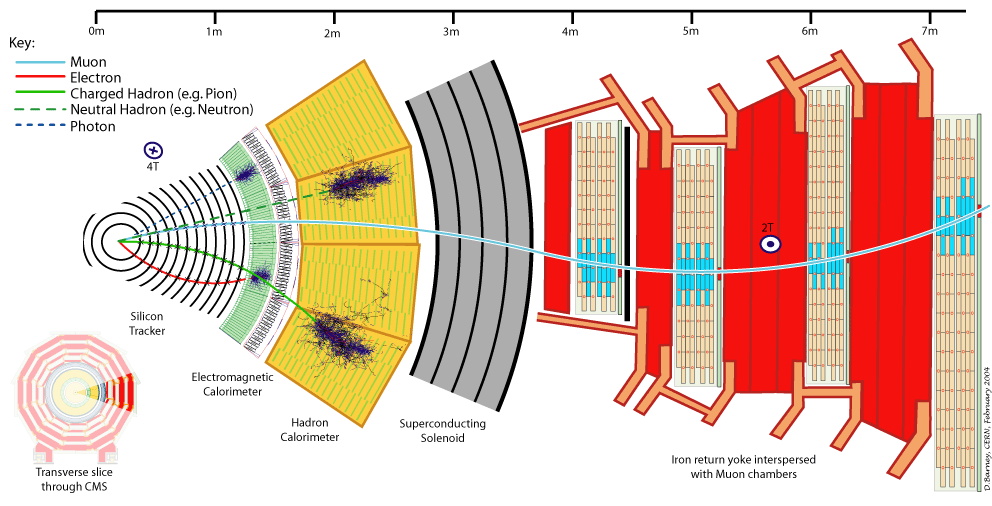
\includegraphics[width=1.0\textwidth]{04_event_reconstruction/plots/CMS_Slice.png}
%   \caption{Track reconstruction using different sub-detector information in combination in Particle Flow algorithm. An actual
%   muon track is shown with a curved blue line, an electron track is red and a charged hadron is solid green.}
%   \label{fig:PFmuons}
% \end{figure}
% 
% The resulting list of particles is used for further jet and missing transverse energy ($E_{T}^{miss}$) construction. 
% 
% The performance of the algorithm was studied with the simulated events \cite{CMS-PAS-PFT-09-001}. Particularly the jet energy
% resolution gain reaches factor 3 for a low transverse momentum region. Furthermore, the angular resolution is improved by factor 2-3.
% 
% A more detailed description of each object reconstruction relevant for this analysis is given in the following sections of this chapter.
% A complete overview of the PF algorithm can be found in \cite{CMS-PAS-PFT-09-001}. 
% 
% 
% %%%%%%%%%%%%%%%%%%%%%%%%%%%%%%%%%%%%%%%%%%%%%%%
% \section{Lepton reconstruction and selection}
% 
% The presence of two leptons, electrons or muons, is required for this analysis. Their reconstruction
% differs a lot due to a huge mass distinction. Thus, the reconstruction of leptons and muons is discussed separately.
% 
% \subsection{Muons reconstruction}
% 
% As it was discussed in section \ref{sec:CMS}, the CMS experiment has a well established setup for the muon reconstruction.
% Muons are the only particles expected to appear in the muon sub-detector system, thus their identification is unambiguous.
% Three techniques of muon reconstruction were implemented:
% 
% \begin{itemize}
%  \item [--] \textit{Standalone}: muons are reconstructed using the information from the muon system only. As 
%  this part of the detector provides a tracking information, a complete set of physical properties needed for the further
%  analysis is recorded.
%  
%  \item [--] \textit{Tracker}: the tracks, reconstructed in the tracking detector only, are assigned as muons in case they 
%  match at least one hit in the muon sub-detector. 
%  
%  \item [--] \textit{Global}: the muons are reconstructed using 
%  the combined fit of tracks from the muon system and from the inner tracker.
% \end{itemize}
% 
% Only the global or tracker muons were used for this analysis. It is more efficient to use the tracker algorithm to reconstruct
% low-momentum muons, but it suffers a lot from the presence of a large number of other particles. The global muons with small momenta
% are dominantly using the tracking detector information for the reconstruction, while starting from $p_{T} \sim \textrm{200 GeV}$
% the muon system data plays a significant role.
% 
% \subsection{Electrons reconstruction}\label{ssec:ElRec}
% 
% To reconstruct the electrons a combined information from the tracking detector and ECAL was used \cite{CMS-PAS-EGM-10-004}. The energy
% deposits in the ECAL are grouped into superclusters\footnote{A \textit{supercluster} is  a group of one or more associated clusters 
% of energy deposits in the ECAL. It is constructed taking into account its characteristic narrow width in the pseudorapidity $\eta$
% and its characteristic spread in $\phi$ due to the bending in the magnetic field of electrons radiating in the tracker material.} 
% with transverse energy $E_{T} > \textrm{4 GeV}$ and fitted to the tracks in the tracking detector \cite{GSF_Electron_Reconstruction_CMS}.
% 
% For a better quality of the tracks a restriction on the impact parameter\footnote{An \textit{impact parameter} $d_{xy}$ of the track is a minimum
% distance of the track to the primary vertex in the transverse $x-y$ plane.} $|d_{xy}| < 0.4 mm$ is applied. A maximum one hit in the inner tracker
% which is positioned close to the track, but not reconstructed, is allowed for the electron candidate.
% 
% On top of the mentioned conditions, a multivariate analysis (MVA) is performed to reduce the number of misidentified electrons.
% 
% \subsection{Lepton selection and isolation}
% 
% Only the events which contain at least two leptons (electrons or muons) with a minimum transverse momentum $p_{T}$ of 20 GeV reconstructed
% in central detector part $|\eta| \leq 2.4$ are accepted for the further analysis.
% 
% To distinguish leptons from hard processes (like a $W^{\pm}$ decay), or \textit{prompt leptons}, from the misidentified charged hadrons 
% and leptons from the jets, an \textit{isolation} criterion is required. The former usually don't overlap with jets, while the latter should
% fly in the same direction and be located in a close vicinity of a jet. This distinction is a basis for the isolation. An energy in a cone 
% around a lepton (not counting the lepton energy itself) is calculated. That is the definition of a combined isolation:
% 
% \begin{equation}
%  I_{comb} = I_{tracker} + I_{ECAL} + I_{HCAL} = \sum E_{photons} + \sum E_{hadrons}
% \end{equation}
% 
% The combined isolation $I_{comb}$ divided by the lepton transverse momentum $p_{T}(l)$ is the relative isolation used as a discriminant value:
% 
% \begin{equation}
%  I_{rel} = \frac{I_{comb}}{p_{T}(l)}
% \end{equation}
% 
% Leptons with the $I_{rel} \leq 0.15$ in the cone $\Delta R = \sqrt{\Delta\eta^{2} + \Delta\phi^{2}} = 0.3$ are selected.
% 
% \subsection{Lepton pair selection}
% 
% The $t\bar{t}$ decay final state has two oppositely charged leptons, while the selected events may contain three or more leptons.
% Out of all the leptons in the event, only the pair of opposite sign tracks with the maximum total transverse momentum $p_{T}(l\bar{l})$
% is selected. After this step the event is tagged with the $t\bar{t}$ decay channel -- $ee$, $e\mu$ or $\mu\mu$.
% 
% To minimize the fraction of the Drell-Yan low-mass resonances only the lepton pairs with the masses higher then 20 GeV are accepted. 
% 
% The same flavour final states ($ee$ and $\mu\mu$) are highly contaminated by the $Z/\gamma * \to ee/\mu\mu$ processes. To lower this effect
% the restriction on the mass window of the lepton pair system $\textrm{76 GeV} \leq m(l\bar{l}) \leq \textrm{106 GeV}$ is applied which removes  
% the mass peak of the $Z-$boson resonance at $\textrm{91 GeV}$. This condition is only required for the $ee$- and $\mu\mu$-tagged events.
% 
% 
% %%%%%%%%%%%%%%%%%%%%%%%%%%%%%%%%%%%%%%%%%%%%%%%
% \section{Jet reconstruction and selection}
% 
% Each $t$ quark from the $t\bar{t}$ decays to a $b$. A quark as a colorful object can't exist singly due to the confinement property (see sec. \ref{sec:quark}).
% A $b$ quark thus starts to hadronize and form a group of particles (primarily hadrons only) flowing in one direction. These are the jets. The LHC proton-proton collisions
% are providing an environment with a fertile hadron activity which makes a jet reconstruction not a straight forward task. Special algorithms are developed
% to find and reconstruct jets.
% 
% \subsection{Jet Finder Algorithms}
% 
% The simple idea which lies behind any algorithm of a jet finding and reconstruction is the merging of the objects which are measured near by in the detector.
% Generally a jet can be reconstructed using two strategies \cite{Salam:2007xv}:
% 
% \begin{itemize}
%  \item \textit{Sequential clustering}: the particles are sequentially recombined until the closest (regarding the actual distance between measured
%  objects) combination is found.
%  %
%  \item \textit{Cone algorithms}: a jet is defined as a cone around some direction of dominant energy flow. Each or some of the particles are tried 
%  in a role of the dominant direction seed. The next step was to define a trial cone around the seed and accept all the particles which enter this cone.
%  The sum of the four-momenta of all objects inside the jet candidate area is calculated and assumed to be a new seed. This iterative process continues
%  until the stable seed is found.
% \end{itemize}
% 
% Although the cone algorithms are fast and simplistic they are not collinear and infrared safe by default. This means that the jets constructed this way will
% change if one of the jet components will face a collinear splitting and do not account for additional soft radiation.
% 
% The sequential clustering algorithms are both infrared and collinear safe, though may be not that fast. They don't rely on a stable cone. The procedure of constructing
% a jet starts with defining two distances -- $d_{ij}$ (the distance between two objects, particles or pseudojets, $i$ and $j$ in the detector) and $d_{iB}$ (the distance between the object $i$
% and the beam). These two distances are compared:
% 
% \begin{itemize}
%  \item [--] $d_{ij} < d_{iB}$: the objects $i$ and $j$ are combined together to a pseudojet which enters the clustering again as a single object;
%  \item [--] $d_{ij} > d_{iB}$: the object $i$ is taken as a final jet.
% \end{itemize}
% 
% The different sequential clustering algorithms differ at the level of the distance definition. In general the distances are defined as follows \cite{Cacciari:2008gp}:
% 
% \begin{align}
%  d_{ij} & = min(k_{Ti}^{2p}, k_{Tj}^{2p}) \frac{\Delta_{ij}^{2}}{R^{2}},\label{eq:ktDist} \\
%  d_{iB} & = k_{Ti}^{2p}, \\
%  \Delta_{ij}^{2} & = (y_{i} - y_{j})^{2} + (\phi_{i} - \phi_{j})^{2}.
% \end{align}
% 
% Here the $k_{Ti}$, $y_{i}$ and $\phi_i$ are the transverse momentum, rapidity and azimuth angle of an object $i$. The $R$ is a cone radius which tells 
% how large the jet can be. A $p$ is the parameter which varies the power of the energy in comparison to the geometrical scale $\Delta_{ij}$.
% The algorithm behaves differently depending on a $p$ value:
% 
% \begin{itemize}
%  \item $p = 1$ defines the $k_{T}$ algorithm, where the energetic and spatial term are of the same power;
%  \item $p = 0$ defines the Cambridge/Aachen algorithm, where the energetic term in eq.\ref{eq:ktDist} is removed thus the spatial part only plays role;
%  \item $p = -1$ defines the anti-$k_{T}$ algorithm which produces circular shaped infrared and collinear safe jets.
% \end{itemize}
% 
% The jets for this analyses were constructed making use of the anti-$k_{T}$ sequential clustering algorithm. The procedure was carried out with real and
% simulated data (on the generator level and after the detector simulation).
% 
% Jets are reconstructed with a particle flow concept (see sec. \ref{sec:PF}) using the information from all the sub-detector parts.
% 
% \subsection{Jet Energy Calibration}\label{ssec:JCal}
% 
% The reconstructed jet energy should be corrected for the non-linear and non-uniform responses of the calorimeter. For this sake a factorized jet calibration
% method is used \cite{2011JInst...611002C}. Calibration is performed sequentially in several steps displayed on the Figure \ref{fig:JECsc}.
% 
% \begin{figure}[h]
%   \centering
%   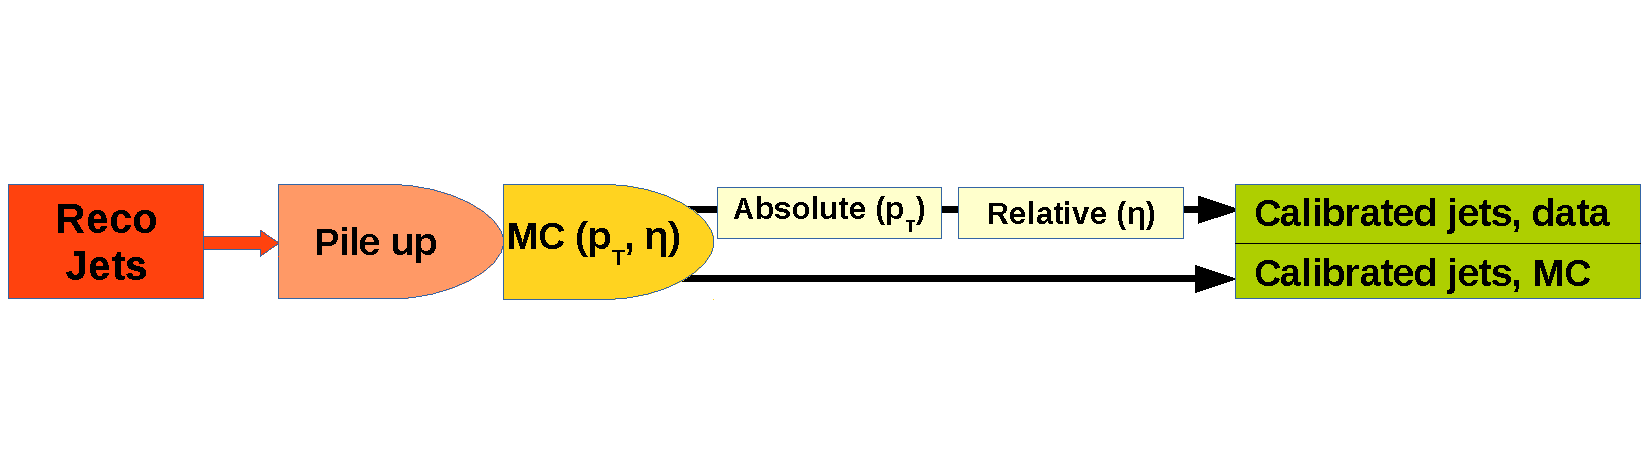
\includegraphics[width=1.0\textwidth]{04_event_reconstruction/plots/JEC.pdf}
%   \caption{Jet calibration steps applied for the detector data and simulated MC samples.}
%   \label{fig:JECsc}
% \end{figure}
% 
% First calibration step deals with the additional energy in the jet which does not occur from a hard process but rather from the detector noise or pile up. 
% Obviously this correction produces the factor always smaller then 1 thus the jet energy reduces on this step. Further correction steps aim to make the jet response
% flat as a function of $|\eta|$ and $p_{T}$. The correction on the geometrical position dependence corrects all the energies as if they were measured 
% in the most efficient barrel region using the dijet data events. The $p_{T}$ dependence correction makes use of the Drell-Yan events to exploit a good
% lepton energy and momentum resolutions. Finally the residual corrections are applied on data to correct for some minor disagreement with the simulation.
% 
% In general all the corrections factor in the kinematic region of interest for this analysis are smaller then $5\%$.
% 
% \subsection{Jet selection}
% 
% This analysis requires only the events where at least two well reconstructed jets are present. All the energies are calibrated as explained in sec.\ref{ssec:JCal}.
% The jets are required to be reconstructed in the barrel region of the detector with the pseudorapidity $|\eta| \leq 2.4$ and with the transverse momentum of at least 
% 30 GeV. 
% 
% \subsection{b-Jets identification}\label{ssec:bTag}
% 
% A jet may arise from any parton, not only from a $b$ quark. But there are some properties which may allow to distinguish a $b$-jet from the other jets. In particular
% a long life time of the B hadrons (in the order of $10^{-12}$ s) allows it to travel far enough from the primary interaction point before the decay. The point
% in space, which corresponds to the place of $B$-hadron decay can be reconstructed in the pixel tracking detector as a \textit{secondary vertex}. The other important
% parameter which can be used to identify the jet origin is the impact parameter of the tracks arising from the secondary vertex. The discussed properties are 
% displayed on the Figure \ref{fig:SV}.
% 
% \begin{figure}[t]
%   \centering
%   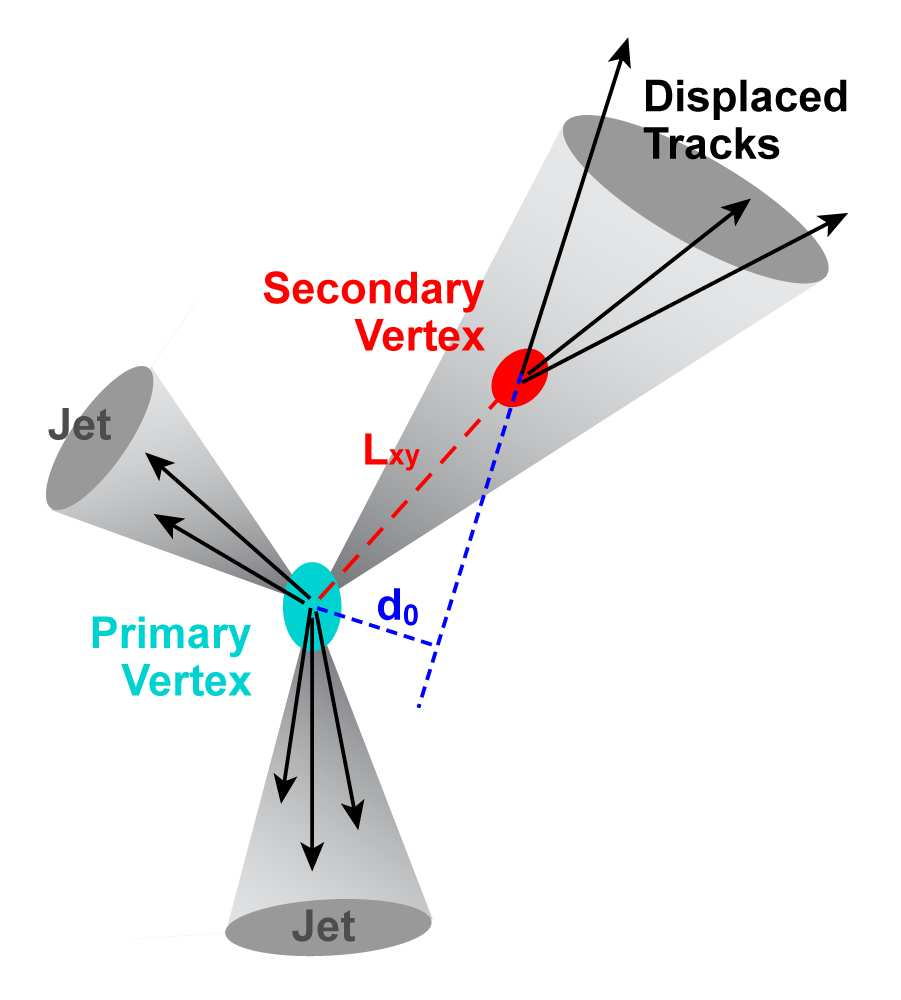
\includegraphics[width=0.5\textwidth]{04_event_reconstruction/plots/btagging_cartoon.png}
%   \caption{A sketch of the event with a reconstructed secondary vertex. A light blue circle is the primary vertex and a red circle is the secondary vertex. The impact 
%   parameter is marked with a blue dashed line and a symbol $d_{0}$.}
%   \label{fig:SV}
% \end{figure}
% 
% The algorithms which aim to find the jets originating from $b$-quarks are called the \textit{b-tagging algorithms}. All of them define a single discriminator value for each jet.
% The algorithms used for the different analyses of the data recored by the CMS detector in 2012 are listed as follows \cite{CMS-PAS-BTV-13-001}: 
% 
% \begin{itemize}
%  \item \textit{Track Counting High Purity} (THCP): the discriminator value is defined as a significance of the impact parameter\footnote{A \textit{significance} is a relation 
%  of the impact parameter value $d$ to it's measurement uncertainty $\sigma_{d}$: $S = \frac{d}{\sigma_{d}}$} of the track with the third highest
%  impact parameter significance;
%  %
%  \item \textit{Jet Probability} (JP): the discriminator is a likelihood value for all associated tracks to arise from the primary vertex. 
%  %
%  \item \textit{Combined Secondary Vertex} (CSV): a likelihood-based discriminator uses the secondary vertex and lifetime information to distinguish $b$-jets, $c$-jets
%  and light jets. This method was exploited for the analyses presented.
% \end{itemize}
% 
% The minimum thresholds for the algorithm are defined as three \textit{working points}, loose (L), medium (M) and tight (T), as following \cite{CMS-PAS-BTV-13-001}:
% 
% \begin{itemize}
%  \item [--] CSVL sets the threshold on the actual discriminator value as $\geq 0.244$, which has an efficiency $\sim 80\%$ and a misidentification probability of
%  light hadron jets close to $10\%$;
%  %
%  \item [--] CSVM sets a harsher threshold on the discriminator value of $\geq 0.679$, which lowers the misidentification probability to $\sim 1\%$, but also
%  reduces the statistics down to 65$\%$;
%  %
%  \item [--] CSVT has the hardest threshold on the discriminator value of $\geq 0.898$. This lowers the misidentification probability by other factor of 10 ($0.1\%$)
%  and reduces the efficiency down to 50$\%$;
% \end{itemize}
% 
% In general the efficiency of the CSV algorithm was estimated in data and simulated QCD events \cite{CMS-PAS-BTV-13-001}. The resulting curve is presenter on the figure \ref{fig:CSVeff}.
% 
% \begin{figure}[t]
%   \centering
%   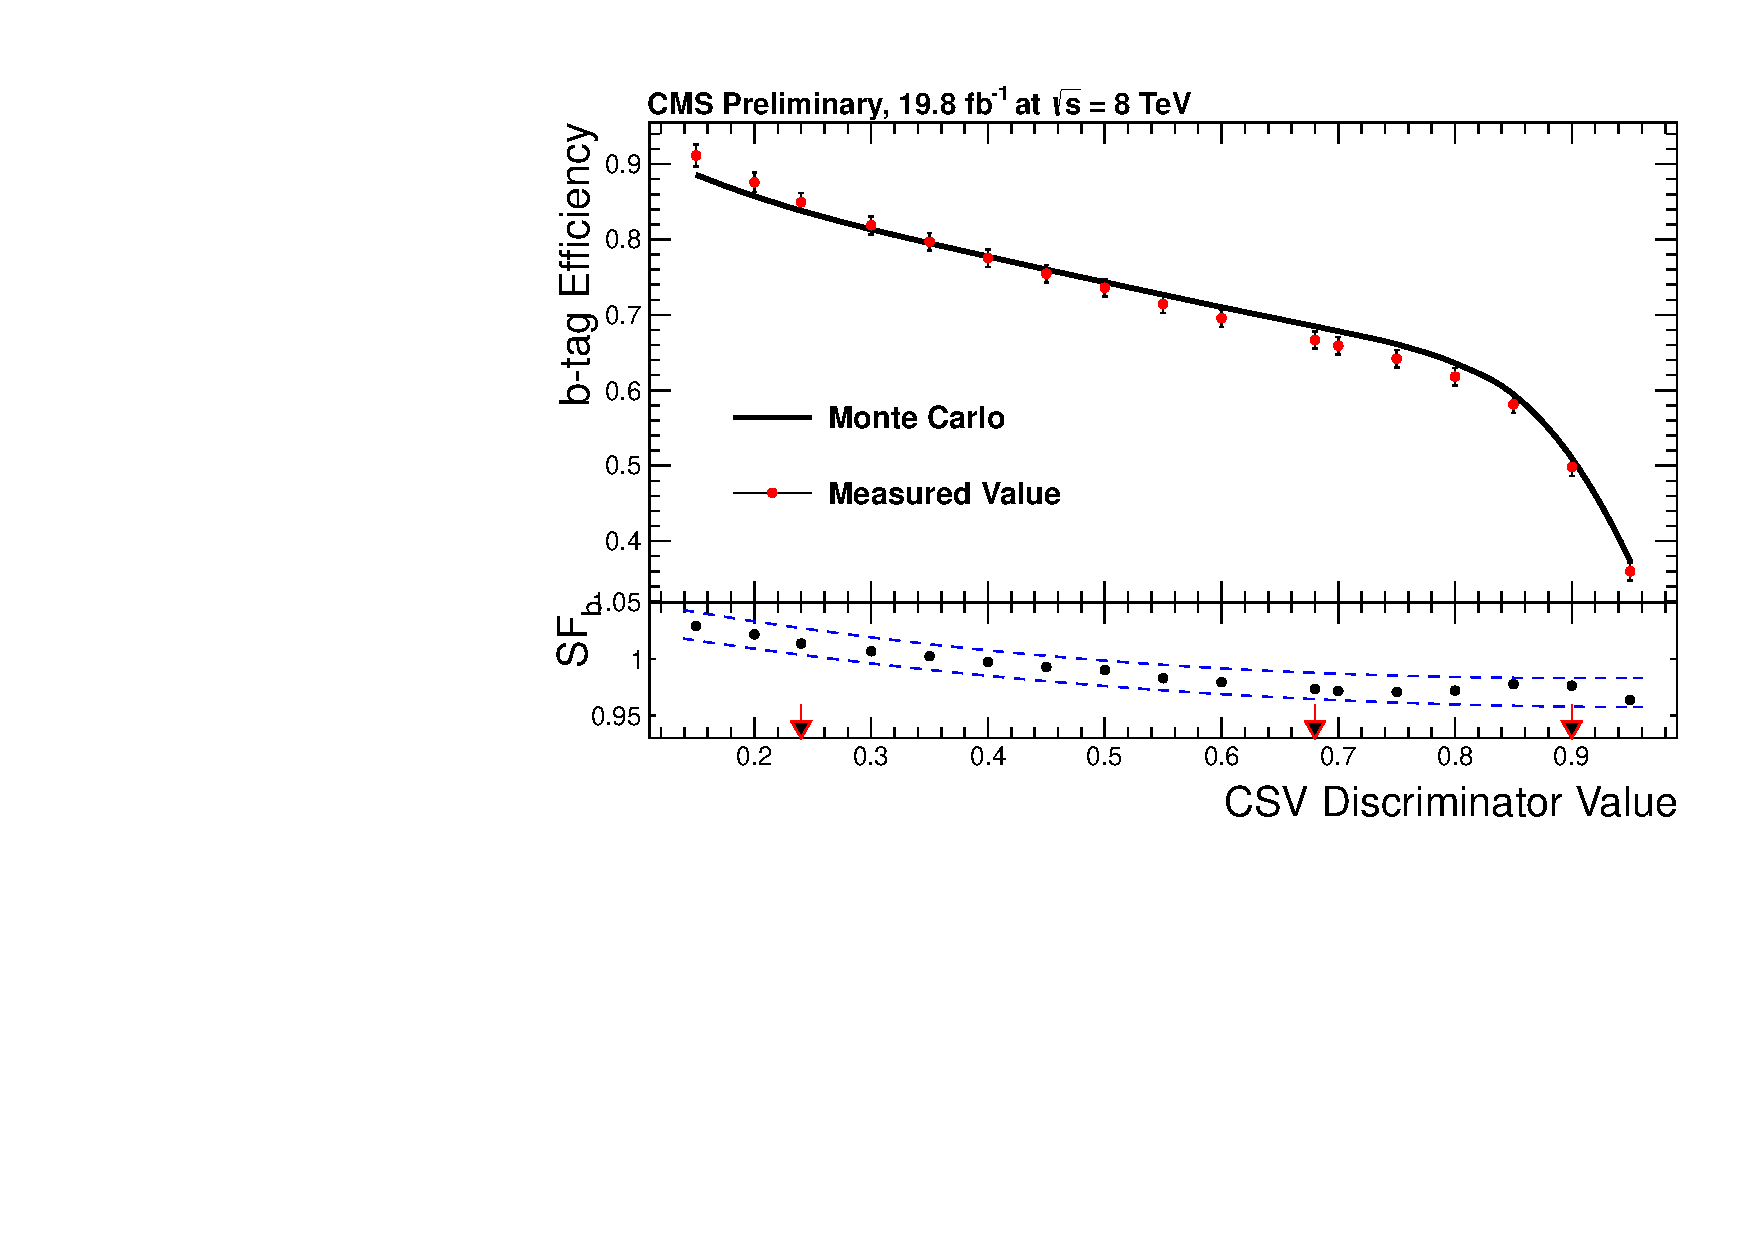
\includegraphics[width=0.6\textwidth]{04_event_reconstruction/plots/Figure_012-b.pdf}
%   \caption{A b-jet tagging efficiency as a function of the discriminator threshold for the CSV algorithm. The upper panel shows the efficiency measured in data and predicted from the simulation.
%   The lower panel shows the ratio between data and simulation efficiencies, where the blue line represents the combined statistical and systematical uncertainty. The plot is taken from \cite{CMS-PAS-BTV-13-001}.}
%   \label{fig:CSVeff}
% \end{figure}
% 
% For this analysis the jets are tagged as arising from a $b$-quark in case they are accepted by CSVL. An event is selected only if it contains at least one $b$-tagged jet.
% 
% \section{Missing Transverse Energy}
% 
% Previously the reconstruction methods and algorithms of all the charged objects of the $t\bar{t}$ dilepton final states were described. However the most complicated 
% task is to reconstruct the two neutrinos which are neutral and don't interact with detector material thus don't provide any direct trace. The only thing to rely on is
% observation of the energy imbalances which may point to the presence of undetected objects. The variable responsible for energy imbalance in the transverse plane is 
% the missing transverse energy $\vec{E^{miss}_{T}}$ (see sec. \ref{sec:CMS}) which is reconstructed using the particle flow algorithm \cite{CMS-PAS-PFT-09-001} (see sec. \ref{sec:PF})
% as a vectorial sum over all reconstructed particles in the event and then taking the opposite of this azimuthal, momentum two-vector. The missing transverse energy is the modulus
% of this vector.
% 
% \begin{align}
%  \vec{E}_{T}^{miss} & = (E_{T_{x}}^{miss}, \, E_{T_{y}}^{miss}) = - \sum_{leptons} \vec{p}_{T}^{lepton} - \sum_{jets} \vec{p}_{T}^{jet}, \\
%  E_{T}^{miss} & = \sqrt{E_{T_{x}}^{miss^{2}} + E_{T_{y}}^{miss^{2}}}.
% \end{align}
% 
% Missing transverse energy reconstruction strongly relies on the quality of leptons and jets reconstruction and is sensitive to the pile up objects. Thus, it is
% crucial to have a precise distinction to the objects from different collisions. To correct for the pile up effects the Multivariate Analysis (MVA) was performed \cite{CMS-PAS-JME-12-002}.
% The MVA is trained on the $Z \to e^{+}e^{-} / \mu^{+}\mu^{-}$ samples and attempts to distinguish between the events emerging from the hard interaction point and
% pile up verteces. The improvement in resolution which the exploiting of the MVA for pile up rejection gives is $\sim 6\%$. However, the differences between data
% and simulation are getting larger. To compensate for these discrepancies the \textit{recoil corrections} are applied \cite{CMS-PAS-JME-12-002}. 
% 
% A recoil $\vec{u}$ is calculated using the well reconstructed $Z \to e^{+}e^{-} / \mu^{+}\mu^{-}$ samples and is defined as shown in the eq. \ref{eq:recoil}:
% 
% \begin{equation}
%  \vec{u} = - \vec{p}_{T}(Z) - \vec{E}_{T}^{miss}
% \end{equation}
% 
% The parallel ($u_{||}$) and perpendicular ($u_{\perp}$) components with respect to the $Z$ direction are simultaneously fitted in data and simulation for each bin
% of the jet multiplicity and $p_{T}(Z)$. The areas of the fit curves $f$ in data and MC simulations are required to be equal:
% 
% \begin{equation}
%  \int_{-\infty}^{u_{corr}} f_{data}\; du = \int_{-\infty}^{u_{uncorr}} f_{sim.}\; du.
% \end{equation}
% 
% The corrected recoil value $u_{corr}$ is used to reestimate the missing transverse energy as $\vec{E}_{T}^{miss} = | \vec{p}_{T}(Z) - \vec{u}_{corr}$.
% 
% For this analysis the events in the $ee$ and $\mu\mu$ channels are accepted only in case the missing transverse energy is $E_{T}^{miss} > 40 \textrm{GeV}$. This rejects
% the background events with a not real missing transverse energy.
% 
% \section{Event Selection Summary}
% 
% The full final state objects selection has been presented and all the selection criteria are summarized as follows:
% 
% \begin{itemize}
%  \item [--] \textbf{Trigger selection}: The events have to be accepted by the dilepton triggers, which require the presents of two leptons, electrons or muons, with
%  minimum transverse momentum of 17 GeV and 8 GeV. 
%  %
%  \item [--] \textbf{Beam scrapping}: Accept only events with maximum 10 reconstructed tracks, or more then 10 in case at least quarter of them has high quality of reconstruction.
%  %
%  \item [--] \textbf{Calorimeter noise removal}: Event with anomalous calorimeter noise are removed.
%  %
%  \item [--] \textbf{Presence of a good vertex}: Events which contain at least one primary vertex with high reconstruction quality are accepted.
%  %
%  \item [--] \textbf{Lepton selection}: An event has to contain at least two leptons with $p_{T} > 20 \textrm{GeV}$ and $|\eta| < 2.4$. Both leptons have to be isolated with 
%  $I_{rel}\leq 0.15$ in a cone of $\Delta R = 0.3$.
%  %
%  \item [--] \textbf{Lepton pair selection}: The mass of the system of two leading $p_{T}$ leptons has to be less then 20 GeV, otherwise the event is rejected. For the
%  same flavour channels a window of $76\textrm{ GeV}\leq m(l\bar{l}) \leq 106\textrm{ GeV}$ is cut out.
%  %
%  \item [--] \textbf{Jet selection}: The events which contain at least two jets with $p_{T} > 30$ GeV and $|\eta| \leq 2.4$ are accepted. Additionally, an event has to contain
%  at least one jet, tagged as originating from the $b$-quark with the help of CSVL.
%  %
%  \item [--] \textbf{Missing Transverse Energy selection}: For the same flavour channels only the events with $E_{T}^{miss} > 40$ GeV are accepted.
% \end{itemize}
% 
% The set of selection criteria performs successfully decreasing the fraction of background events. The control distributions which show the data and MC simulation at one plot
% contain all the background sources as a part of MC, thus providing a visualization of the outcoming results of the event selection process. 